\documentclass[11pt]{article}
\usepackage{icmlko}
\begin{document}

\title{두 번째 수집 회차가 축 하나를 벗겼다 --- 시장팝업의 절반은 ``기자가 적었나''였다}
\author{월드모델 실험실}
\date{노트 354 · 2026년 8월 1일}
\maketitle

\begin{abstract}
노트 353이 지목한 것을 했다 --- 시장팝업 유보를 늘린다. 원인을 찾다가
\textbf{일곱 번째 갈라진 목록}이 나왔다. ``ingest/market\_axes.build'' 의
첫 줄이 \texttt{not d.get("single\_event")} 로 거르는데, \textbf{MKT2 배치
239건은 그 칸이 한 번도 안 쓰였다}(239/239 \texttt{None}). ``단일 행사가
아니어서''가 아니라 ``칸이 비어서'' 배치 통째로 떨어지고 있었다 --- 축
파일 205행이 전부 MKT 인 것이 그 자국이다. 규칙으로 메워 44행을
되살렸다(유보 $104\to126$).

미리 적어 둔 위험이 켜졌다. 새 배치는 \texttt{is\_free\_entry} ·
\texttt{reservation\_required} 가 \textbf{0/44} 라 \texttt{entry\_friction}
표시자가 MKT $0.79$ 대 MKT2 $0.00$ --- 표시자가 곧 배치다. 사전 등록대로
막았다. 그리고 갈라 보니 \textbf{그 축이 나르던 것은 값이 아니라
결측이었다}: 관측된 행 안에서 값과 라벨의 (연도 통제) $\rho$ 는 학습
$+0.0233$ · 유보 $+0.0664$ 인데, ``적혔나''와 라벨은 $+0.1859$ ·
$\mathbf{+0.2362}$ 다. 시장팝업 $\rho$ 0.2761 중 0.1577 이 \emph{그 취재가
자세했나}였다. 지금 시장팝업은 $0.1365$, 95\% $[-0.029,\,0.321]$ ---
\textbf{0 을 못 배제한다.} 대신 못 가리는 쌍이 $35\to29$ 로, 한 번에
제일 크게 줄었다.
\end{abstract}

\section{일곱 번째 갈라진 목록}

노트 335부터 여섯 번 같은 모양을 잡았다 --- 거르는 쪽 · 긁는 쪽 둘 ·
읽는 쪽 둘 · 만드는 쪽 하나가 서로 다른 목록을 보고 있었다. 일곱 번째다.

\begin{center}
\begin{tabular}{lrrl}
\hline
배치 & 레코드 & 축에 쓰임 & \texttt{single\_event} \\
\hline
MKT  & 408 & \textbf{205} & True 309 · False 99 \\
MKT2 & 239 & \textbf{0}   & \textbf{None 239} \\
\hline
\end{tabular}
\end{center}

\begin{center}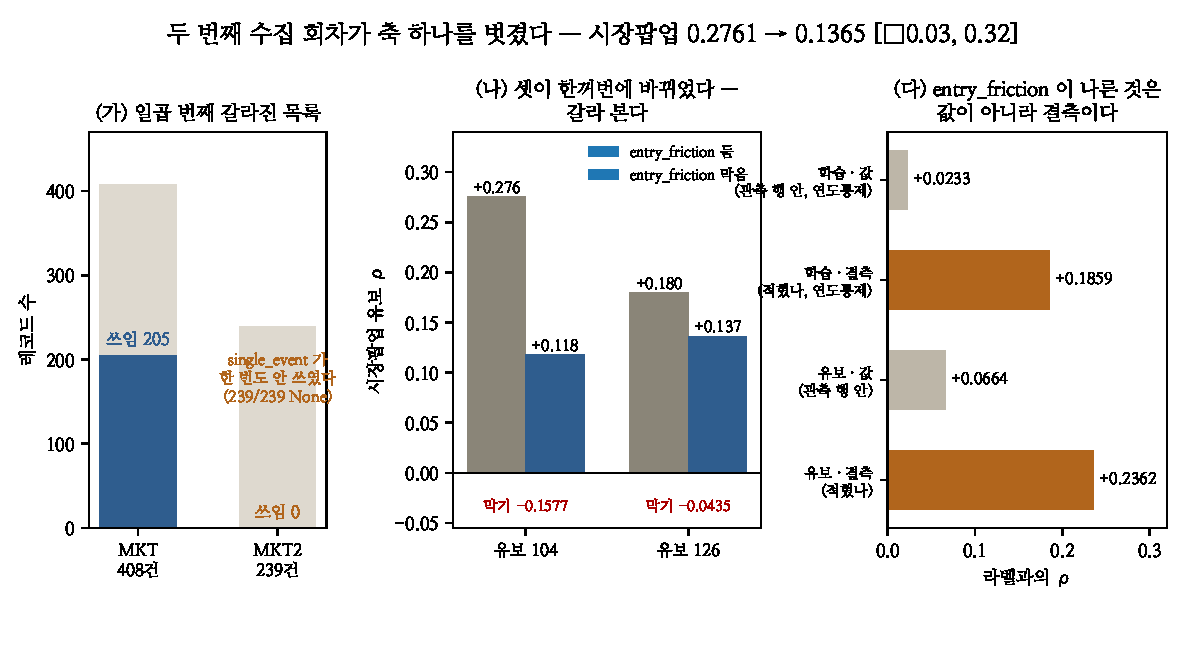
\includegraphics[width=\linewidth]{figs/batch.pdf}\end{center}

떨어진 것 중 라벨 · 기간 · 등급이 멀쩡한 46건은 \texttt{multi\_store} 가
전부 \texttt{False} 이고 \texttt{\_aggregate} · \texttt{exclude\_reason} 도
없다 --- 마뗑킴 롯데백화점 부산점 · 원신 신촌 · W컨셉 성수 · 빵빵이
더현대. 평범한 단일 팝업이다.

\textbf{레코드별로 보고 정하지 않았다.} 칸이 비었으면 규칙으로 메운다 ---
여러 점포가 아니고, 집계도 아니고, 제외 사유도 없으면 단일 행사다.
44행이 붙었다(학습 $101\to123$ · 유보 $104\to126$).

\section{미리 적어 둔 위험이 켜졌다}

사전 등록에 이렇게 적었다.

\begin{quote}
제일 큰 위험은 \textbf{표시자가 배치를 나르는} 것이다(노트 326의 풀
그림자). \texttt{poolshadow} 를 돌려 확인한다. \textbf{갈라지면 그 축들을
시장팝업에서 뺀다.}
\end{quote}

갈라졌다. \texttt{entry\_friction} 표시자가 MKT $0.79$ 대 MKT2
$\mathbf{0.00}$ 이다. MKT2 레코드는 \texttt{is\_free\_entry} 와
\texttt{reservation\_required} 칸이 \emph{있는데 전부 \texttt{null}} 이다
(0/44) --- 읽기 실수가 아니라 수집 구멍이다. 막았다
(\texttt{lab/fixaxes.BLOCK}).

\textbf{라벨 쪽은 통과했다.} 노트 353의 새 규약대로 연도를 맞춰 봤다 ---
중앙값이 2023년 $3.14/3.31$ · 2024년 $3.18/2.85$ · 2025년 $3.14/3.23$ ·
2026년 $3.00/3.24$ 이고 유보 맨휘트니 $p=0.148$ 이다. 두 배치는 같은
것을 재고 있다.

\section{셋이 한꺼번에 바뀌었다 --- 갈라 본다}

행이 늘고(학습·유보 둘 다), 축 하나가 막혔다. 노트 133의 규약대로 갈랐다.

\begin{center}
\begin{tabular}{lrrr}
\hline
시장팝업 $\rho$ & \texttt{entry} 둠 & \texttt{entry} 막음 & 막기의 값 \\
\hline
MKT2 뺌 (유보 104)   & $+0.2761$ & $+0.1184$ & $\mathbf{-0.1577}$ \\
MKT2 넣음 (유보 126) & $+0.1800$ & $+0.1365$ & $-0.0435$ \\
\hline
MKT2 의 값           & $-0.0961$ & $+0.0181$ & \\
\hline
\end{tabular}
\end{center}

\textbf{비싼 것은 새 행이 아니라 막기다.} 그리고 막기의 값이 두 줄에서
$3.6$ 배 다르다 --- 옛 유보 104행에는 MKT2 가 없어서 그 축이 배치
표시자가 \emph{아니고}, 거기서 막으면 순수한 손해다. 배치가 섞인 뒤에는
$-0.0435$ 로 줄어든다.

\section{그 축이 나르던 것}

그래서 물었다 --- \texttt{entry\_friction} 은 무엇으로 벌었나. 노트 266이
애니 \texttt{air\_quarter} 에서 쓴 방법 그대로, \emph{관측된 행 안에서만}
다시 잰다.

\begin{center}
\begin{tabular}{lrr}
\hline
 & 학습 & 유보 \\
\hline
\textbf{값} --- 관측 행 안, 연도 통제 & $+0.0233$ (n=72) & $+0.0664$ (n=89) \\
\textbf{결측} --- ``적혔나'', 연도 통제 & $+0.1859$ (n=101) & $\mathbf{+0.2362}$ (n=104) \\
\hline
\end{tabular}
\end{center}

\textbf{값에는 아무것도 없다.} 신호는 통째로 ``기사에 입장료나 예약
여부가 적혀 있었나''다. 그것은 그 행사가 얼마나 자세히 취재됐나이고,
자세히 취재되는 것은 큰 행사다. \textbf{시장팝업 $\rho$ 0.2761 중
0.1577 이 취재 밀도였다.}

이것을 \emph{두 번째 수집 회차가} 드러냈다. 한 배치만 있을 때는 관측률
79\%가 그냥 결측처럼 보인다. 두 번째 배치가 0\%로 들어오자 ``표시자가
배치다''라는 질문이 강제됐고, 그 질문을 따라가니 첫 배치 안에서도 값이
아니라 결측이 벌고 있었다. \textbf{배치를 하나 더 모으는 것은 행을
늘리는 일이기만 한 것이 아니다 --- 축을 감사하는 일이다.}

\section{지금 자리}

\begin{center}
\begin{tabular}{lrr}
\hline
 & 전 (노트 353) & 지금 \\
\hline
시장팝업 $\rho$      & $0.2761$ & $\mathbf{0.1365}$ \\
시장팝업 95\%        & $[0.085,\,0.468]$ & $\mathbf{[-0.029,\,0.321]}$ \\
시장팝업 유보        & 104 & 126 \\
판                   & $0.4877$ & $0.4814$ \\
판 분모              & 2,695 & 2,717 \\
\textbf{못 가리는 쌍}& 35 & $\mathbf{29}$ \\
\hline
\end{tabular}
\end{center}

\textbf{긴 갈래 하나가 닫힌다.} 노트 285부터 ``시장팝업이 왜 자꾸 지나''를
물어 왔고 노트 351이 서랍을 비웠고 노트 352가 ``진다는 전제부터 안
재졌다''고 했다. 이제 126행으로 재면 답이 나온다 --- \textbf{시장팝업의
신호는 0 과 못 가른다.} 그 도메인의 축들이 못 미친 것이 아니라, 있던
$0.28$ 중 절반 이상이 취재 밀도였고 나머지는 표본 잡음과 안 갈린다.

그리고 이번에도 점수는 내려가고 재는 힘은 올라간다 --- 노트 353과 같은
방향이다. 못 가리는 쌍이 $35\to29$ 로, 한 번에 제일 크게 줄었다.

\section{규약에 더하는 줄}

\begin{itemize}
\item \textbf{배치가 둘 이상이면 축마다 배치별 표시자율을 본다.} 한
배치에서 79\%, 다른 배치에서 0\% 인 축은 축이 아니라 수집 회차다.
\item \textbf{표시자가 벌면 값이 버는지 따로 잰다.} 노트 266이 애니에서
한 것을 모든 도메인에 건다 --- 시장팝업에서 두 번째로 걸렸다.
\item \textbf{새 배치는 축 감사다.} 행을 늘리려고 모은 배치가 기존 축의
정체를 밝힌다. 이번엔 시장팝업 $\rho$ 의 절반이었다.
\end{itemize}

\section{남은 것}

\begin{center}
\begin{tabular}{ll}
\hline
갈래 & 지금 아는 것 \\
\hline
결측이 버는 축이 또 있나 & 시장팝업에서 걸렸다. 열 도메인 전 축에 \\
                        & 같은 검사를 돌린다. \textbf{다음 순번} \\
MKT2 나머지 195건 & 라벨 · 기간이 없다. 다시 뽑으면 유보가 더 는다 \\
MKT2 입장/예약 0/44 & 원문에서 다시 뽑으면 축이 되살아난다 \\
추가 2026 아홉 행 & 노트 353. 아이돌 라벨 수준이 한터와 반대 \\
\hline
\end{tabular}
\end{center}

첫 줄이 다음이다. 이 판에 축이 서른아홉 개인데 그중 몇이 결측으로 벌고
있는지 아무도 센 적이 없다.

\end{document}
